%-----------------------------------------------------------------
%	PRESENTATION BODY
%	!TEX root = ./presentation.tex
%-----------------------------------------------------------------
\section{Objectives}
\begin{frame}{Objectives}
	\begin{itemize}
		\item Analysis of the influence of the SST on tropical-cyclones intensity.
		\begin{list}{\textcolor{mygreen}{$\circ$}}{}
			\item Replicate the results obtained by \citeauthor{Corral2010} in~\cite{Corral2010}.
			\item Update these results with revised data.
		\end{list}
		\item Analysis regarding the influence of the SST, or lack thereof, on the intensity and duration of tropical-cyclones.
	\end{itemize}
\end{frame}

%-----------------------------------------------------------------
\section{Introduction}

\subsection{Tropical-cyclones tracks}
\begin{frame}{Tropical-cyclones tracks}

\begin{onlyenv}<1>
\only<1>{\frametitle{Tropical-cyclones tracks}}
\begin{figure}[H]
	\centering
	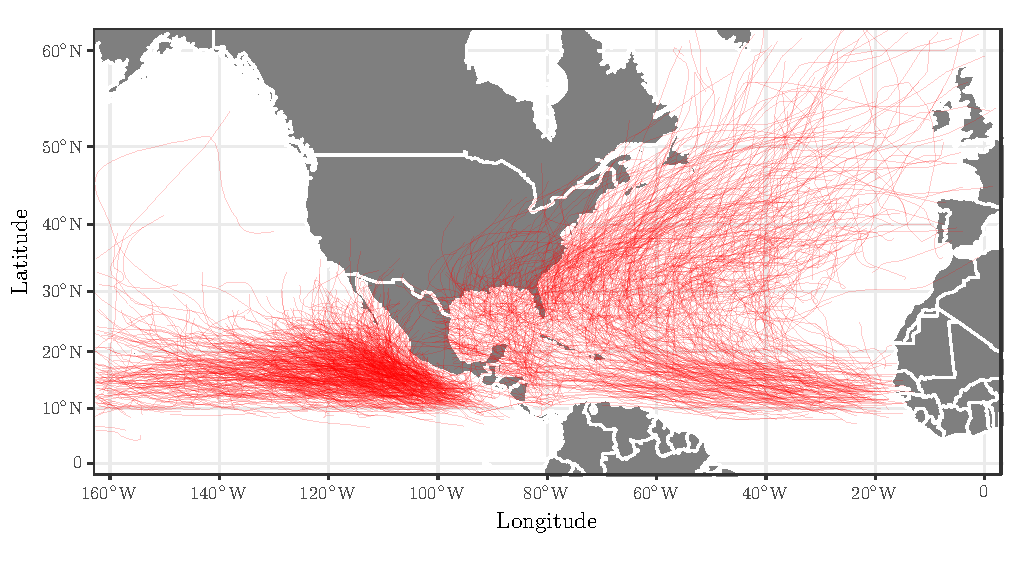
\includegraphics[scale=0.6]{images/complete-map}
	\caption{Tropical-cyclones tracks for the Northeast Pacific (E.~Pac.) \& North Atlantic (N.~Atl.) Oceans}
	\label{fig:figure1}
\end{figure}
% \end{frame}
\end{onlyenv}

\begin{onlyenv}<2>
% \begin{frame}{Individual storm intensity}
\only<2>{\frametitle{Individual storm intensity}}
\vspace{-0.9cm}
\begin{columns}[c] % align columns
	\begin{column}{.65\textwidth}
	\begin{figure}[H]
		\centering
		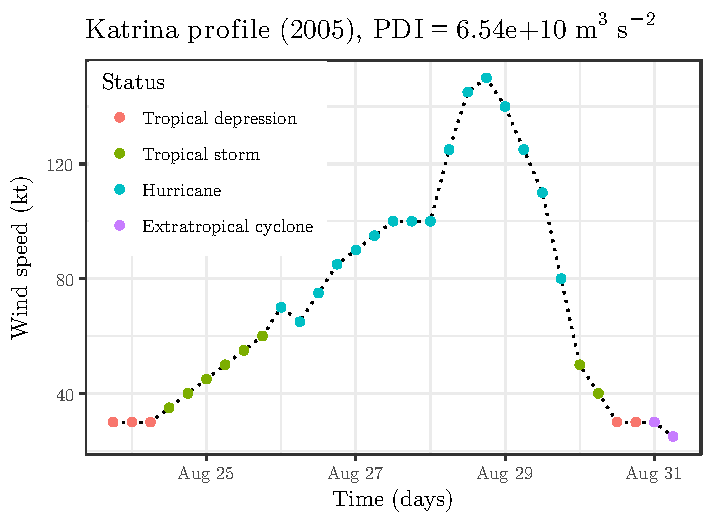
\includegraphics[scale=0.6]{images/track-storm-katrina}
		\caption{Katrina surface wind speed profile}
		\label{fig:figure1}
	\end{figure}
	\end{column}%
	\hfill%
	\begin{column}{.35\textwidth}
	\begin{align}\label{eq:pdi-bis}
		PDI = \sum_{t} v_{t}^{3} \Delta t
	\end{align}
	\end{column}%
\end{columns}
\end{onlyenv}

\end{frame}

\subsection{Probability density distribution}
\begin{frame}{\emph{D(PDI)} distribution}
\begin{figure}[H]
	\centering
	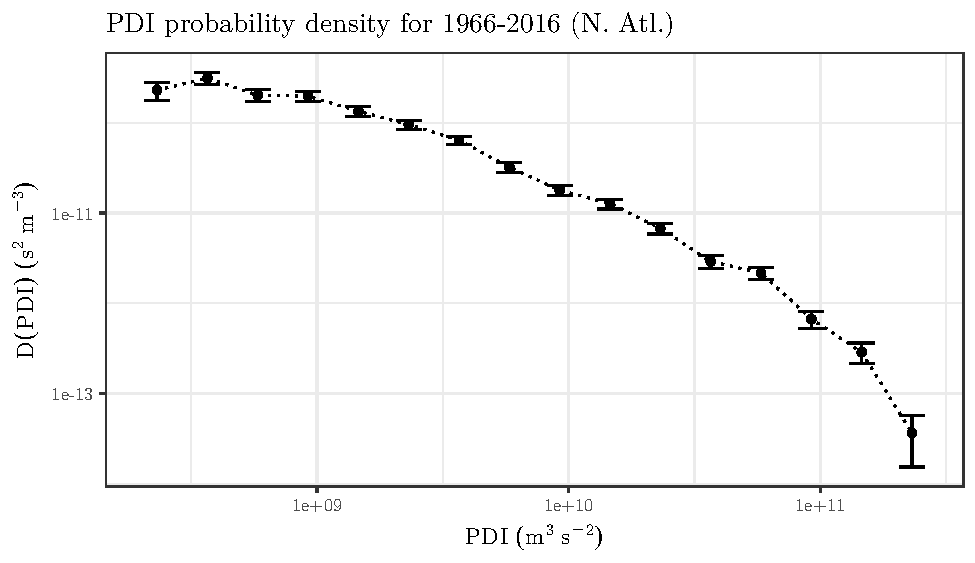
\includegraphics[scale=0.6]{images/dpdi-natl}
	\caption{$D(PDI)$ distribution for the North Atlantic Ocean}
	\label{fig:figure1}
\end{figure}
\end{frame}

%-----------------------------------------------------------------
\section{Analyses}
\subsection{Separation by SST}

\begin{frame}<1>[label=analyses]{Analyses}
\begin{itemize}[<+>]
	\item \textbf{Separation by SST}

	\begin{onlyenv}<1>
		Higher SSTs and increased water vapour $\to$ high-SST years should have a longer tail.
	\end{onlyenv}
	\item \textbf{PDI correlations}

	\begin{onlyenv}<2>
		Why do high-SST years have more energetic tropical-cyclones?
		Once cyclones are activated, they should behave the same regardless of the SST.
	\end{onlyenv}
\end{itemize}
\end{frame}


%-----------------------------------------------------------------
\begin{frame}{Separation by SST}
\frametitle<3>{Results}
\begin{figure}[H]
	\centering
	\vspace{-0.3cm}
	\includegraphics<1>[scale=0.75]{images/map-sst-cont}
	\includegraphics<2>[scale=0.6]{images/sst-analysis-natl}
	\includegraphics<3>[scale=0.6]{images/dpdi-by-class-natl}
	\caption{\only<1>{Global SST (in \si{\celsius}) map from May 2017} %
			 \only<2>{SST analysis for the North Atlantic Ocean} %
			 \only<3>{$D(PDI)$ distributions calculated separately for years with high or low SST for the North Atlantic Ocean} }
	\label{fig:figure1}
\end{figure}
\end{frame}

%-----------------------------------------------------------------
\subsection{PDI correlations}
\againframe<2>{analyses}

\begin{frame}{PDI correlations}
\begin{figure}[H]
	\centering
	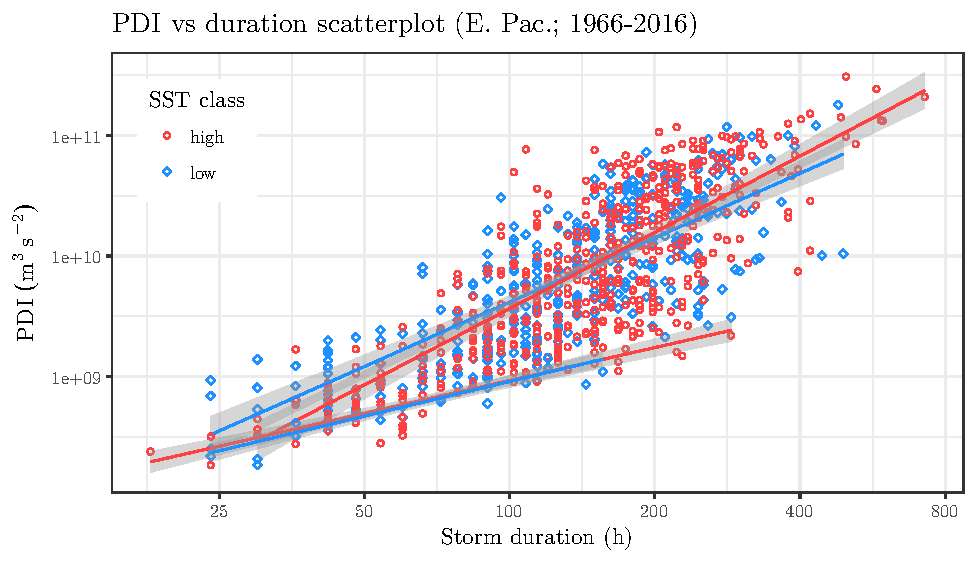
\includegraphics[scale=0.6]{images/scatter-epac-ds}
	\caption{$PDI$ vs duration analysis for non-developing and developing systems for the Northeast Pacific Ocean}
	\label{fig:figure1}
\end{figure}
\end{frame}

%-----------------------------------------------------------------
\section{Conclusions}
\begin{frame}{Conclusions}
\begin{itemize}
	\item<1-> Corroboration of global warming.
	\item<1-> An example of its severe consequences.
\end{itemize}
\begin{list}{\textcolor{mygreen}{$\Plus$}}{}
	\item<2> Comprehensive study of all basins.
	\item<2> Individual SST tracking per storm (ICOADS).
	\item<2> Multivariate statistics for the correlation analyses.
\end{list}
\end{frame}

%-----------------------------------------------------------------
\appendix
\begin{frame}{References}
% \begin{frame}[allowframebreaks]{References}
	\def\newblock{}
	\nocite{Corral2010}
	\nocite{Webster2005}
	\nocite{Emanuel2003}
	\printbibliography[heading=bibintoc]
\end{frame}
